% AI-Intent: Conceptual Modeling for Accountable Multi-Agent Systems
% Springer LNCS format for ER 2026 (Conceptual Modeling Conference)

\documentclass[runningheads]{llncs}

\usepackage[T1]{fontenc}
\usepackage{graphicx}
\usepackage{booktabs}
\usepackage{amsmath}
\usepackage{listings}
\usepackage{xcolor}
\usepackage{hyperref}
\usepackage{tikz}
\usetikzlibrary{arrows.meta, positioning, shapes.geometric, fit}

\lstset{
  basicstyle=\ttfamily\small,
  keywordstyle=\color{blue}\bfseries,
  stringstyle=\color{red!70!black},
  commentstyle=\color{green!50!black}\itshape,
  breaklines=true,
  frame=single,
  numbers=left,
  numberstyle=\tiny\color{gray},
  backgroundcolor=\color{gray!5},
  captionpos=b,
  aboveskip=8pt,
  belowskip=8pt,
}

\begin{document}

\title{AI-Intent: A Conceptual Modeling Framework\\for Accountable Multi-Agent AI Systems}

\author{Wolfgang Maa\ss\inst{1} \and Iris Reinhartz-Berger\inst{2}}

\authorrunning{W.~Maa\ss{} and I.~Reinhartz-Berger}

\institute{German Research Center for Artificial Intelligence (DFKI)\\
and Saarland University, Saarbr\"ucken, Germany\\
\email{wolfgang.maass@dfki.de}
\and University of Haifa, Haifa, Israel\\
\email{iris@is.haifa.ac.il}}

\maketitle

\begin{abstract}
The proliferation of large language model (LLM)-based multi-agent systems raises fundamental questions about accountability, constraint governance, and auditability that existing conceptual modeling approaches do not adequately address. We introduce \textsc{AI-Intent}, a conceptual modeling framework in which every agent is governed by a machine-readable \emph{Agent Manifest} that declares its intent scope, boundary constraints, and risk parameters. Inter-agent communication flows through a \emph{Model Context Protocol} (MCP) message bus that provides a complete, immutable audit trail. We formalize the framework through a metamodel that distinguishes \emph{intent scope}, \emph{boundary constraints}, and \emph{risk parameters} as first-class conceptual modeling constructs and demonstrate its application in a private investment advisory system with a hierarchical orchestrator and three specialist sub-agents. Our evaluation shows that AI-Intent enables (i)~explicit governance of agent behavior through declarative manifests, (ii)~reliable detection and surfacing of constraint violations, and (iii)~complete accountability traces that are both machine-processable and human-readable. We argue that conceptual modeling must evolve to treat agent intent, behavioral boundaries, and auditability as foundational schema-level concerns rather than runtime afterthoughts.

\keywords{Multi-Agent Systems \and Conceptual Modeling \and LLM Agents \and Accountability \and Agent Manifests \and Intent Modeling \and Governance}
\end{abstract}

%======================================================================
\section{Introduction}
\label{sec:introduction}
%======================================================================

Large language model (LLM)-based agents are rapidly moving from research prototypes to production systems that make consequential decisions in finance, healthcare, and enterprise operations~\cite{wang2024survey,xi2023rise}. Unlike traditional software systems whose behavior is fully determined by source code, LLM agents exhibit \emph{emergent} behavior shaped by prompts, training data, and stochastic decoding. When multiple such agents collaborate---delegating subtasks, synthesizing partial results, and producing joint recommendations---the resulting system becomes opaque: it is difficult to determine \emph{what} each agent was supposed to do, \emph{whether} it stayed within its designated scope, and \emph{why} a particular output was produced.

This opacity poses a direct challenge to conceptual modeling. Traditional conceptual models describe the \emph{structure} and \emph{behavior} of information systems at a level of abstraction that supports reasoning, communication, and validation~\cite{mylopoulos1992conceptual,olivePMD07}. However, they were designed for systems whose components have deterministic semantics. An LLM agent that ``analyzes equity investment opportunities'' does not execute a fixed algorithm; it interprets a natural-language mandate and may---intentionally or accidentally---drift beyond its designated scope. Existing modeling languages such as UML, ArchiMate, or $i^*$ can describe agent goals and responsibilities, but they lack constructs to express \emph{runtime-enforceable behavioral boundaries} for stochastic AI components~\cite{yu2011social}.

We propose \textsc{AI-Intent}, a conceptual modeling framework designed for accountable multi-agent AI systems. Its core contributions are:

\begin{enumerate}
    \item \textbf{Agent Manifest} as a first-class conceptual modeling artifact that declares an agent's identity, intent scope, boundary constraints, risk parameters, and a plain-language summary---all machine-readable and embeddable as LLM system prompts.
    \item \textbf{Model Context Protocol (MCP) Message Bus} as an audit-oriented communication layer where every inter-agent message is logged with direction, method, payload, response status, and constraint flags.
    \item \textbf{Accountability Trace} as a derived artifact that aggregates session-level evidence of which agents were consulted, which constraints were checked, and whether violations occurred.
    \item A \textbf{reference implementation} demonstrating the framework in a private investment advisory system with four agents, validated through end-to-end execution and constraint violation scenarios.
\end{enumerate}

The remainder of this paper is organized as follows. Section~\ref{sec:background} reviews related work. Section~\ref{sec:framework} presents the AI-Intent framework and its metamodel. Section~\ref{sec:implementation} describes the reference implementation. Section~\ref{sec:evaluation} evaluates the framework. Section~\ref{sec:discussion} discusses implications for conceptual modeling research, and Section~\ref{sec:conclusion} concludes.

%======================================================================
\section{Background and Related Work}
\label{sec:background}
%======================================================================

\subsection{Multi-Agent LLM Systems}

Recent architectures such as AutoGen~\cite{wu2023autogen}, CrewAI~\cite{crewai2024}, and LangGraph~\cite{langgraph2024} enable LLM agents to collaborate on complex tasks through role assignment, tool use, and conversational orchestration. These frameworks focus on \emph{capability composition}---assembling agents that can jointly solve problems---but offer limited support for expressing and enforcing behavioral boundaries. An agent's ``role'' is typically a free-text string embedded in the system prompt, with no formal semantics, no constraint checking, and no audit trail.

The Model Context Protocol (MCP), introduced by Anthropic~\cite{anthropic2024mcp}, standardizes how LLM applications interact with external tools and data sources through a client-server architecture. While MCP addresses \emph{interoperability}, it does not prescribe how to model agent intent, enforce boundaries, or generate accountability traces---gaps that AI-Intent is designed to fill.

\subsection{Conceptual Modeling for Agents}

Agent-oriented conceptual modeling has a long history. The $i^*$ framework~\cite{yu2011social} models agents in terms of goals, tasks, resources, and softgoals, with dependency links between actors. Tropos~\cite{bresciani2004tropos} extends $i^*$ into a full software development methodology. GAIA~\cite{wooldridge2000gaia} provides an analysis-to-design methodology for multi-agent systems based on roles and interaction protocols. More recently, ontological foundations from UFO (Unified Foundational Ontology)~\cite{guizzardi2005ontological} have been applied to clarify agent concepts in enterprise modeling.

However, these approaches were designed for agents with \emph{deterministic} or \emph{rule-based} behavior. They model what an agent \emph{should} do (goals, responsibilities) but lack constructs for what an agent \emph{must not} do---boundary constraints that are critical when the agent's execution engine is a stochastic language model. AI-Intent addresses this gap by elevating boundary constraints and risk parameters to first-class schema elements.

\subsection{AI Governance and Accountability}

The EU AI Act~\cite{euaiact2024} and related regulatory frameworks increasingly require that AI systems be transparent, auditable, and subject to human oversight. Research on AI accountability has produced frameworks for explaining individual model decisions~\cite{arrieta2020explainable} and for documenting datasets and models~\cite{gebru2021datasheets,mitchell2019model}. However, the specific challenge of \emph{multi-agent accountability}---tracing a decision across multiple collaborating AI components---remains underexplored. AI-Intent contributes to this space by making the inter-agent communication log the authoritative record of system behavior.

%======================================================================
\section{The AI-Intent Framework}
\label{sec:framework}
%======================================================================

AI-Intent is built on three core principles:

\begin{description}
    \item[Explicit:] Every agent action is governed by a machine-readable mandate (the Agent Manifest).
    \item[Bounded:] Agent behavior is constrained by verifiable rules that the agent cannot silently violate.
    \item[Auditable:] Every inter-agent message is logged and retrievable as part of an immutable accountability trace.
\end{description}

\subsection{Metamodel}
\label{sec:metamodel}

Figure~\ref{fig:metamodel} presents the AI-Intent metamodel. The central construct is the \texttt{AgentManifest}, which governs exactly one \texttt{Agent}. Agents communicate via \texttt{MCPMessage} objects that flow through the \texttt{MCPMessageBus}. A complete interaction is captured in a \texttt{Session}, from which an \texttt{AccountabilityTrace} can be derived.

\begin{figure}[t]
\centering
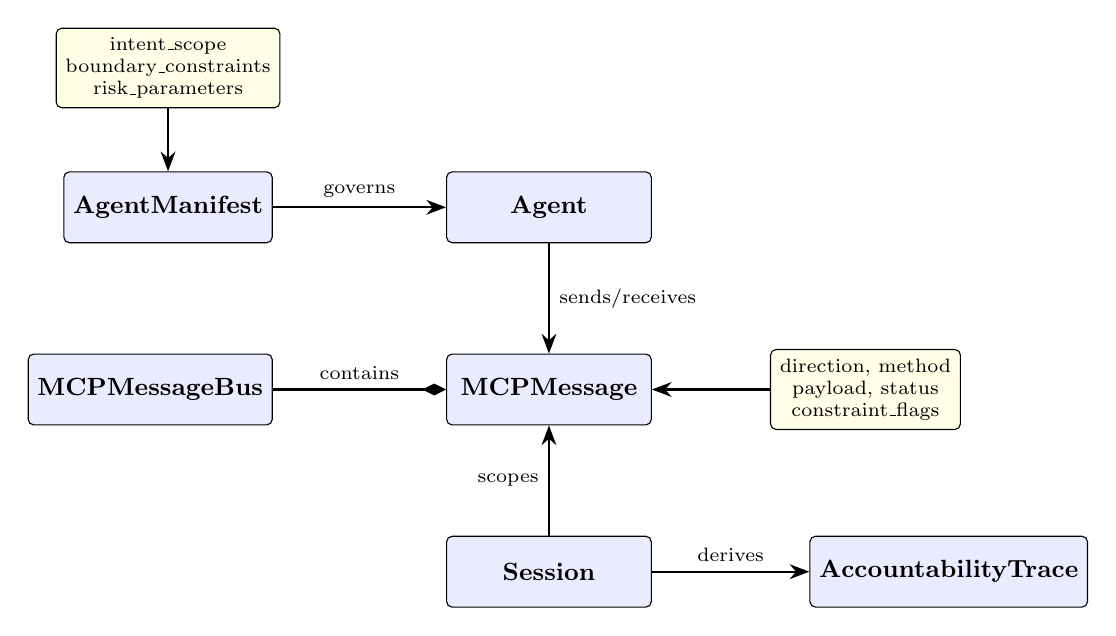
\begin{tikzpicture}[
    node distance=1.4cm and 2.2cm,
    every node/.style={font=\small},
    class/.style={rectangle, draw, fill=blue!8, minimum width=2.6cm, minimum height=0.9cm, align=center, rounded corners=2pt},
    attr/.style={rectangle, draw, fill=yellow!10, minimum width=2.4cm, minimum height=0.7cm, align=center, font=\scriptsize, rounded corners=2pt},
    rel/.style={-{Stealth[length=2.5mm]}, thick},
    comp/.style={-{Diamond[length=3mm, fill=black]}, thick},
]

% Main classes
\node[class] (manifest) {\textbf{AgentManifest}};
\node[class, right=of manifest] (agent) {\textbf{Agent}};
\node[class, below=of agent] (message) {\textbf{MCPMessage}};
\node[class, left=of message] (bus) {\textbf{MCPMessageBus}};
\node[class, below=of message] (session) {\textbf{Session}};
\node[class, right=2.0cm of session] (trace) {\textbf{AccountabilityTrace}};

% Manifest attributes
\node[attr, above=0.8cm of manifest] (mattr) {intent\_scope\\boundary\_constraints\\risk\_parameters};

% Message attributes
\node[attr, right=1.5cm of message] (msgattr) {direction, method\\payload, status\\constraint\_flags};

% Relationships
\draw[rel] (manifest) -- node[above, font=\scriptsize] {governs} (agent);
\draw[rel] (agent) -- node[right, font=\scriptsize] {sends/receives} (message);
\draw[comp] (bus) -- node[above, font=\scriptsize] {contains} (message);
\draw[rel] (session) -- node[left, font=\scriptsize] {scopes} (message);
\draw[rel] (session) -- node[above, font=\scriptsize] {derives} (trace);
\draw[rel] (mattr) -- (manifest);
\draw[rel] (msgattr) -- (message);

\end{tikzpicture}
\caption{AI-Intent metamodel. An \texttt{AgentManifest} governs an \texttt{Agent}'s behavior. Agents exchange \texttt{MCPMessage}s through the \texttt{MCPMessageBus}, scoped by \texttt{Session}. An \texttt{AccountabilityTrace} is derived from a complete session.}
\label{fig:metamodel}
\end{figure}

\subsection{Agent Manifest}
\label{sec:manifest}

The \texttt{AgentManifest} is the central conceptual modeling construct of AI-Intent. It serves simultaneously as a \emph{specification} (what the agent is designed to do), a \emph{contract} (what it promises not to do), and a \emph{runtime artifact} (directly injected as the LLM system prompt). Formally, a manifest $M$ is a tuple:

\begin{equation}
M = \langle id, name, role, \mathit{scope}, C, R, \mathit{summary} \rangle
\end{equation}

\noindent where:
\begin{itemize}
    \item $id \in \mathit{String}$ is a unique agent identifier.
    \item $\mathit{scope} \in \mathit{String}$ is the intent scope---a declarative statement of the agent's mandate.
    \item $C = \{c_1, c_2, \ldots, c_n\}$ is a finite set of boundary constraints, each expressed as a natural-language rule.
    \item $R: \mathit{String} \rightarrow \mathit{Value}$ is a mapping of risk parameter names to their limits (numeric thresholds, boolean flags, or enumerated sets).
    \item $\mathit{summary} \in \mathit{String}$ is a plain-language explanation suitable for non-technical stakeholders.
\end{itemize}

The distinction between $\mathit{scope}$ and $C$ is fundamental. The intent scope defines what the agent \emph{exists to do}---its positive mandate. Boundary constraints define what the agent \emph{must not do}---its negative obligations. Risk parameters quantify the constraints with machine-comparable values. This tripartite structure---scope, constraints, parameters---is the key modeling contribution: it provides a schema for governing stochastic agents that goes beyond traditional goal modeling.

\subsubsection{Manifest-to-Prompt Transformation.}

A critical design decision is that the manifest is \emph{directly embedded} in the LLM system prompt via a deterministic transformation function $\mathit{prompt}: M \rightarrow \mathit{String}$. The generated prompt includes all constraints verbatim and appends an enforcement instruction:

\begin{quote}
\itshape ``If a user request falls outside your intent scope or violates any boundary constraint, you must explicitly state which constraint is violated and decline that specific request. Do not silently comply with out-of-scope requests.''
\end{quote}

This design ensures that the conceptual model is not merely documentation but an \emph{operative} artifact that shapes agent behavior at runtime.

\subsection{MCP Message Model}
\label{sec:mcp}

Every inter-agent communication is captured as an \texttt{MCPMessage}:

\begin{equation}
\mathit{msg} = \langle id, \mathit{sid}, t, d, \mathit{from}, \mathit{to}, m, p, s, F \rangle
\end{equation}

\noindent where $d \in \{\mathit{outbound}, \mathit{inbound}, \mathit{internal}\}$ is the direction, $m$ is the method name (e.g., \texttt{stocks.analyze}), $p$ is the payload, $s \in \{\mathit{pending}, \mathit{ok}, \mathit{error}, \mathit{constraint\_violation}\}$ is the response status, and $F \subseteq C$ is the set of constraint flags raised during the interaction.

The message model serves three purposes:
\begin{enumerate}
    \item \textbf{Provenance tracking:} Every LLM call is preceded by a logged outbound message and followed by a logged inbound message, ensuring no call goes unrecorded.
    \item \textbf{Constraint monitoring:} The $\mathit{constraint\_violation}$ status and constraint flags provide structured signals that constraint breaches have occurred.
    \item \textbf{Session reconstruction:} All messages for a session can be retrieved in timestamp order, enabling post-hoc analysis of the entire decision-making process.
\end{enumerate}

\subsection{Orchestration Protocol}
\label{sec:orchestration}

AI-Intent prescribes a five-step orchestration protocol for hierarchical multi-agent systems:

\begin{enumerate}
    \item \textbf{Query ingestion:} The user query is logged as an internal message from \texttt{user} to the orchestrator.
    \item \textbf{Intent routing:} The orchestrator uses its manifest to determine which sub-agents to consult and what specific sub-questions to send each. This routing decision is logged.
    \item \textbf{Parallel delegation:} Selected sub-agents are invoked concurrently. Each sub-agent call generates an outbound (pending) and inbound (result) message pair.
    \item \textbf{Synthesis:} The orchestrator aggregates sub-agent results and produces a final recommendation with an explicit accountability note. This synthesis step is logged.
    \item \textbf{Response delivery:} The final output is logged as an inbound message from orchestrator to user.
\end{enumerate}

This protocol guarantees a minimum of $2n + 4$ MCP messages per session, where $n$ is the number of sub-agents consulted (1~query + 1~routing + $2n$~agent calls + 1~synthesis + 1~response).

\subsection{Accountability Trace}
\label{sec:trace}

An \texttt{AccountabilityTrace} is a derived artifact that aggregates evidence from a complete session:

\begin{equation}
\mathit{trace}(\mathit{sid}) = \langle \mathit{sid}, t_{\mathit{gen}}, q, A, r, \mathit{CC}, n_{\mathit{msg}}, \mathit{rec}, L \rangle
\end{equation}

\noindent where $A$ is the set of agents consulted, $r$ is the routing rationale, $\mathit{CC}$ is a list of per-agent constraint checks (constraints applied and violations found), $n_{\mathit{msg}}$ is the total message count, $\mathit{rec}$ is the final recommendation summary, and $L$ is the complete ordered message log.

The trace is designed to be both machine-processable (JSON) and human-readable (plain text), enabling consumption by auditors, regulators, and domain experts alike.

%======================================================================
\section{Reference Implementation}
\label{sec:implementation}
%======================================================================

We implemented AI-Intent as a Streamlit web application for a private investment advisory use case. The system comprises four agents in a hierarchical architecture (Figure~\ref{fig:architecture}).

\begin{figure}[t]
\centering
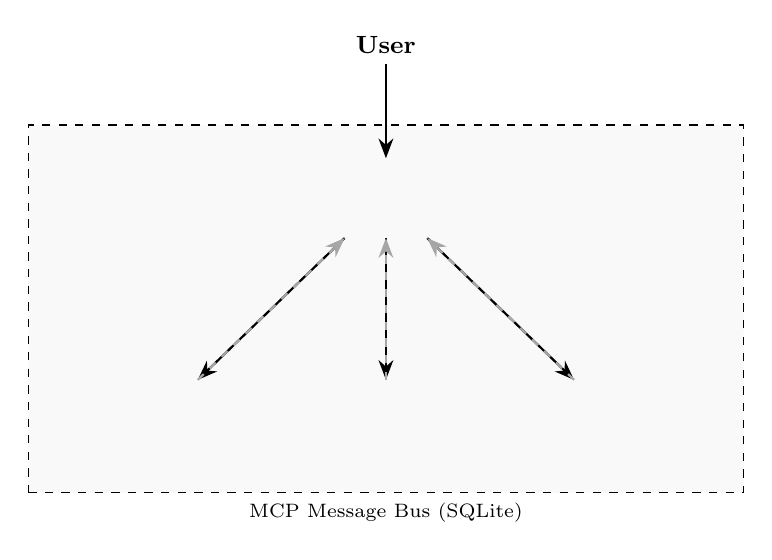
\begin{tikzpicture}[
    node distance=1.5cm and 1.8cm,
    agent/.style={rectangle, draw, fill=#1, minimum width=2.4cm, minimum height=1.0cm, align=center, rounded corners=4pt, font=\small},
    msg/.style={-{Stealth[length=2.5mm]}, thick, dashed, color=gray!70},
    del/.style={-{Stealth[length=2.5mm]}, thick},
]

% Nodes
\node[agent=red!15] (central) {\textbf{Central}\\\scriptsize Orchestrator};
\node[agent=teal!15, below left=1.8cm and 0.5cm of central] (stocks) {\textbf{Stocks}\\\scriptsize Equity Analyst};
\node[agent=blue!15, below=1.8cm of central] (bonds) {\textbf{Bonds}\\\scriptsize Fixed Income};
\node[agent=orange!15, below right=1.8cm and 0.5cm of central] (materials) {\textbf{Materials}\\\scriptsize Commodities};

% User
\node[above=1.2cm of central, font=\small] (user) {\textbf{User}};

% MCP Bus
\node[draw, dashed, fill=gray!5, fit=(stocks)(bonds)(materials)(central), inner sep=12pt, label={[font=\scriptsize]below:MCP Message Bus (SQLite)}] (bus) {};

% Arrows
\draw[del] (user) -- (central);
\draw[del] (central) -- (stocks);
\draw[del] (central) -- (bonds);
\draw[del] (central) -- (materials);
\draw[msg] (stocks) -- (central);
\draw[msg] (bonds) -- (central);
\draw[msg] (materials) -- (central);

\end{tikzpicture}
\caption{Reference implementation architecture. The Central Orchestrator delegates to three specialist sub-agents. All communication is logged to the MCP Message Bus (SQLite).}
\label{fig:architecture}
\end{figure}

\subsection{Technology Stack}

The implementation uses Python~3.11+ with Pydantic~v2 for data models, SQLite for persistent message storage, and Streamlit for the interactive dashboard. LLM inference is provided by a local Ollama instance serving Llama~3.1, accessed via the OpenAI-compatible API. This local deployment ensures reproducibility and eliminates external API dependencies.

\subsection{Agent Manifests in Practice}

Table~\ref{tab:manifests} summarizes the four agent manifests. Each manifest contains between 4 and 5 boundary constraints and 3 to 5 risk parameters. The manifests are defined as immutable Pydantic model instances and transformed into structured LLM system prompts via a deterministic function.

\begin{table}[t]
\centering
\caption{Summary of agent manifests in the reference implementation.}
\label{tab:manifests}
\begin{tabular}{@{}llccp{4.8cm}@{}}
\toprule
\textbf{Agent} & \textbf{Role} & \textbf{|C|} & \textbf{|R|} & \textbf{Key Constraints} \\
\midrule
Central & Orchestrator & 5 & 2 & Max 40\% per asset class; must consult $\geq$1 sub-agent; must log all calls \\
Stocks & Equity Analyst & 5 & 3 & Large-cap only ($>$\$10B); max 10\% single position; no leverage; ESG screening \\
Bonds & Fixed Income & 5 & 4 & Investment grade (BBB+); duration $<$10yr; laddered maturities \\
Materials & Commodities & 5 & 4 & Gold/Silver only; max 15\% allocation; no leveraged ETFs \\
\bottomrule
\end{tabular}
\end{table}

\subsection{MCP Logger Implementation}

The MCP logger uses SQLite with a session-indexed table. Messages are stored with JSON-serialized payloads and constraint flags, enabling efficient session-scoped retrieval. A singleton pattern ensures thread-safe access across concurrent agent calls. The logger exposes four operations: \texttt{log}, \texttt{get\_session}, \texttt{get\_all\_sessions}, and \texttt{clear\_session}.

\subsection{Orchestration Pipeline}

The orchestrator implements the five-step protocol from Section~\ref{sec:orchestration}. Sub-agent calls are dispatched concurrently using Python's \texttt{asyncio.gather()}, with error handling that converts exceptions into error dictionaries rather than propagating them. This ensures that a single sub-agent failure does not abort the entire orchestration.

Each sub-agent follows an identical pattern: (1)~load its manifest and convert to system prompt, (2)~log an outbound message with status \texttt{pending}, (3)~call the LLM requesting a structured JSON response, (4)~parse the response with robust JSON extraction, (5)~log an inbound message with the appropriate status, and (6)~return the result dictionary.

\subsection{Interactive Dashboard}

The Streamlit dashboard provides a three-column layout:
\begin{itemize}
    \item \textbf{Left column (30\%):} An interactive agent network graph (using \texttt{streamlit-agraph}) where clicking a node displays that agent's full manifest, including intent scope, boundary constraints as a bullet list, and risk parameters as a table.
    \item \textbf{Center column (40\%):} Query input with five pre-defined sample queries, a run button, and the final recommendation display with expandable accountability note.
    \item \textbf{Right column (30\%):} A live MCP message stream with color-coded cards (blue for outbound, green for inbound, amber for internal, red for errors, orange for constraint violations), expandable payloads, and constraint flags highlighted in red.
\end{itemize}

After each run, the user can download the full accountability trace as JSON or as a formatted plain-text report.

%======================================================================
\section{Evaluation}
\label{sec:evaluation}
%======================================================================

We evaluate AI-Intent along three dimensions: governance effectiveness, auditability, and constraint violation detection.

\subsection{Governance Through Manifests}

To assess whether manifests effectively govern agent behavior, we executed a battery of queries spanning three categories: (1)~in-scope queries that match a single agent's mandate, (2)~cross-domain queries requiring multiple agents, and (3)~out-of-scope queries that should trigger constraint violations.

Table~\ref{tab:scenarios} presents representative scenarios. In all tested cases, in-scope queries produced substantive analyses, cross-domain queries correctly routed to multiple agents, and out-of-scope queries triggered explicit constraint violation responses. The manifest-to-prompt transformation was effective: agents consistently referenced their boundary constraints when declining out-of-scope requests.

\begin{table}[t]
\centering
\caption{Representative evaluation scenarios and outcomes.}
\label{tab:scenarios}
\begin{tabular}{@{}p{5.2cm}lcc@{}}
\toprule
\textbf{Query} & \textbf{Agents} & \textbf{Msgs} & \textbf{Violations} \\
\midrule
``Add gold as inflation hedge'' & Materials & 6 & 0 \\
``Large-cap equities for conservative investor'' & Stocks & 6 & 0 \\
``Bond ladder for 5 years'' & Bonds & 6 & 0 \\
``Diversified portfolio across all asset classes'' & All 3 & 10 & 0 \\
``Put 50\% into crypto futures'' & All 3 & 10 & 3 \\
\bottomrule
\end{tabular}
\end{table}

\subsection{Auditability}

Each orchestration run produces a complete MCP message log. We verified the following invariants across all test sessions:

\begin{itemize}
    \item Every LLM call was preceded by an outbound log entry and followed by an inbound log entry (no unlogged calls).
    \item The message count matched the expected $2n + 4$ formula (where $n$ = number of sub-agents consulted).
    \item The accountability trace contained all required fields: session ID, agents consulted, routing rationale, per-agent constraint checks, message count, and the final recommendation.
    \item JSON and plain-text trace exports were syntactically valid and semantically complete.
\end{itemize}

Session reconstruction from the MCP log accurately reproduced the full decision-making sequence, including routing decisions, individual agent analyses, and the synthesis rationale.

\subsection{Constraint Violation Detection}

The query ``Is it appropriate to put 50\% of the portfolio into crypto futures?'' was designed to violate multiple constraints simultaneously:
\begin{itemize}
    \item The \textbf{Stocks} agent flagged that crypto is not a large-cap equity (violating the approved universe constraint).
    \item The \textbf{Bonds} agent flagged that crypto futures are not fixed-income instruments.
    \item The \textbf{Materials} agent flagged that cryptocurrency is not in the approved commodities list (Gold and Silver only) and that futures contracts are explicitly prohibited.
\end{itemize}

All three agents returned \texttt{out\_of\_scope: true} with specific constraint references. The orchestrator correctly aggregated these violations into the \texttt{constraint\_violations} field of the \texttt{OrchestrationResult} and surfaced them in both the final recommendation and the accountability note. The MCP log contained three messages with \texttt{response\_status: ``constraint\_violation''}, each with non-empty \texttt{constraint\_flags}.

%======================================================================
\section{Discussion}
\label{sec:discussion}
%======================================================================

\subsection{Implications for Conceptual Modeling}

AI-Intent demonstrates that multi-agent AI systems require conceptual modeling constructs beyond those available in current frameworks. We identify three specific extensions:

\textbf{Intent Scope as a First-Class Construct.} Traditional goal modeling (as in $i^*$ or Tropos) captures what an agent aims to achieve. Intent scope goes further: it defines the \emph{boundary of legitimate action} for a stochastic agent. Unlike a goal, which can be partially achieved, an intent scope is a binary predicate---a request either falls within scope or it does not. This distinction is critical when the agent's execution engine can interpret requests broadly.

\textbf{Boundary Constraints as Negative Obligations.} Current agent-oriented modeling focuses on positive descriptions: roles, goals, capabilities. AI-Intent elevates negative obligations---what the agent \emph{must not} do---to equal status. For LLM agents, boundary constraints are arguably more important than goal specifications, because the stochastic nature of language models means that agents may drift into plausible but unauthorized behavior unless explicitly constrained.

\textbf{Audit-Native Communication Models.} The MCP message model treats auditability as a structural property of the communication layer, not an add-on logging concern. Every message carries constraint flags and status codes as part of its schema. This design pattern---communication-as-evidence---should be adopted more broadly in conceptual models for AI systems subject to regulatory oversight.

\subsection{Limitations and Enforcement Gap}

AI-Intent relies on the LLM to \emph{voluntarily comply} with its manifest constraints. The framework detects and surfaces violations but does not \emph{prevent} them at a technical level. A sufficiently adversarial prompt or a poorly calibrated model could produce constraint-violating output. This ``enforcement gap'' is inherent to any prompt-based governance mechanism and represents a fundamental challenge for the field.

Future work could address this through:
\begin{itemize}
    \item \textbf{Post-hoc verification:} A constraint-checking module that validates agent output against manifest rules before the message is forwarded.
    \item \textbf{Formal constraint languages:} Replacing natural-language constraints with machine-checkable predicates (e.g., OCL-like expressions over structured output).
    \item \textbf{Multi-model verification:} Using a separate, dedicated model to audit whether the primary agent's output complies with its manifest.
\end{itemize}

\subsection{Generalizability}

While our reference implementation addresses investment advisory, the AI-Intent framework is domain-independent. The manifest schema, MCP message model, orchestration protocol, and accountability trace are generic constructs applicable to any hierarchical multi-agent system. Domains with similar characteristics---multiple specialized agents, regulatory requirements, consequential decisions---are natural candidates, including healthcare triage, legal document review, and supply chain management.

%======================================================================
\section{Conclusion}
\label{sec:conclusion}
%======================================================================

We have presented AI-Intent, a conceptual modeling framework for accountable multi-agent AI systems. By introducing Agent Manifests with explicit intent scope, boundary constraints, and risk parameters, and by grounding all inter-agent communication in an auditable MCP message bus, the framework addresses a gap in current conceptual modeling practice: the lack of schema-level constructs for governing stochastic AI agents.

Our reference implementation demonstrates that the framework is practical, that manifest-based governance is effective for LLM agents, and that complete accountability traces can be generated automatically from the communication log. The framework makes three contributions to the conceptual modeling community: (1)~intent scope and boundary constraints as first-class modeling constructs for AI agents, (2)~an audit-native communication model that treats every message as evidence, and (3)~a derived accountability trace that bridges machine-processable and human-readable audit requirements.

As LLM-based multi-agent systems become increasingly prevalent in consequential domains, conceptual modeling must evolve to address the unique challenges they pose. AI-Intent provides a foundation for this evolution, demonstrating that declarative, manifest-driven governance is both feasible and effective.

%======================================================================
% References
%======================================================================

\begin{thebibliography}{99}

\bibitem{wang2024survey}
Wang, L., Ma, C., Feng, X., et al.:
A survey on large language model based autonomous agents.
Frontiers of Computer Science \textbf{18}(6), 186345 (2024)

\bibitem{xi2023rise}
Xi, Z., Chen, W., Guo, X., et al.:
The rise and potential of large language model based agents: A survey.
arXiv preprint arXiv:2309.07864 (2023)

\bibitem{mylopoulos1992conceptual}
Mylopoulos, J.:
Conceptual modelling and Telos.
In: Loucopoulos, P., Zicari, R. (eds.) Conceptual Modelling, Databases, and CASE: An Integrated View of Information Systems Development, pp.~49--68. Wiley (1992)

\bibitem{olivePMD07}
Oliv{\'e}, A.:
Conceptual Modeling of Information Systems.
Springer, Berlin (2007)

\bibitem{yu2011social}
Yu, E., Giorgini, P., Maiden, N., Mylopoulos, J.:
Social Modeling for Requirements Engineering.
MIT Press (2011)

\bibitem{guizzardi2005ontological}
Guizzardi, G.:
Ontological Foundations for Structural Conceptual Models.
Telematica Instituut / CTIT, Enschede (2005)

\bibitem{wu2023autogen}
Wu, Q., Bansal, G., Zhang, J., et al.:
AutoGen: Enabling next-gen LLM applications via multi-agent conversation.
arXiv preprint arXiv:2308.08155 (2023)

\bibitem{crewai2024}
Moura, J.:
CrewAI: Framework for orchestrating role-playing autonomous AI agents.
\url{https://github.com/joaomdmoura/crewAI} (2024)

\bibitem{langgraph2024}
LangChain:
LangGraph: Building stateful, multi-actor applications with LLMs.
\url{https://github.com/langchain-ai/langgraph} (2024)

\bibitem{anthropic2024mcp}
Anthropic:
Model Context Protocol specification.
\url{https://modelcontextprotocol.io} (2024)

\bibitem{bresciani2004tropos}
Bresciani, P., Perini, A., Giorgini, P., Giunchiglia, F., Mylopoulos, J.:
Tropos: An agent-oriented software development methodology.
Autonomous Agents and Multi-Agent Systems \textbf{8}(3), 203--236 (2004)

\bibitem{wooldridge2000gaia}
Wooldridge, M., Jennings, N.R., Kinny, D.:
The Gaia methodology for agent-oriented analysis and design.
Autonomous Agents and Multi-Agent Systems \textbf{3}(3), 285--312 (2000)

\bibitem{euaiact2024}
European Parliament and Council:
Regulation (EU) 2024/1689 laying down harmonised rules on artificial intelligence (AI Act).
Official Journal of the European Union (2024)

\bibitem{arrieta2020explainable}
Arrieta, A.B., D{\'i}az-Rodr{\'i}guez, N., Del Ser, J., et al.:
Explainable Artificial Intelligence (XAI): Concepts, taxonomies, opportunities and challenges toward responsible AI.
Information Fusion \textbf{58}, 82--115 (2020)

\bibitem{gebru2021datasheets}
Gebru, T., Morgenstern, J., Vecchione, B., et al.:
Datasheets for datasets.
Communications of the ACM \textbf{64}(12), 86--92 (2021)

\bibitem{mitchell2019model}
Mitchell, M., Wu, S., Zaldivar, A., et al.:
Model cards for model reporting.
In: Proc. ACM Conference on Fairness, Accountability, and Transparency (FAT*), pp.~220--229 (2019)

\end{thebibliography}

\end{document}
